\chapter{Dictionary Learning}
%\thispagestyle{empty}
In \prettyref{sec:dicts} we give a general definition of dictionaries 
as indexed sets of signal atoms with a unknown structure of the atoms.
Dictionaries for sparse coding of images are indexed collections of vectors with
discrete pixel data. A linear combination of a sparse selection of those
discrete pixel atoms is used to reconstruct signals. 

\section{Structure}
Atoms not just consist of random pixel data. Dictionary atoms also capture
structures that are useful for sparse coding. Just picking a few atoms should
lead to a good reconstruction. 

Finding the right structures for a specific signal is a complex task.
Two main strategies for generation of dictionaries are design or
learning.

\subsection{Designed atoms}
The basis transformations first presented in \prettyref{sec:history} can also
be interpreted as atoms of discrete pixel data. Atoms with only
locality in the frequency domain like cosine from DCT or atoms with both
locality in time and frequency domain like wavelets.
\prettyref{fig:generated_atoms} shows some examples for such
dictionaries. 


\begin{figure}
\centering
\subfloat[cosine]{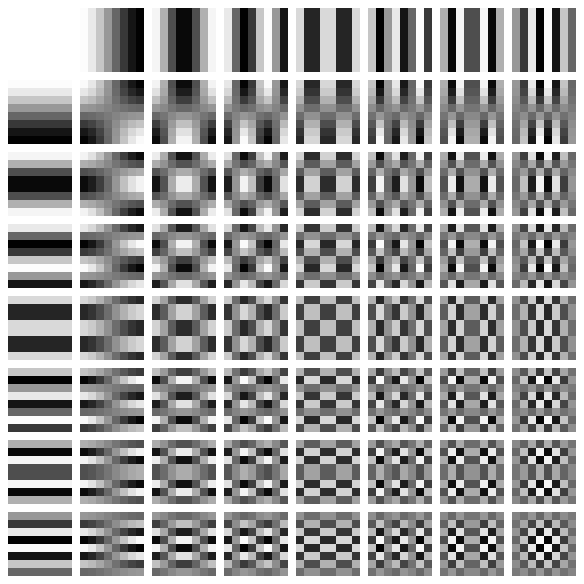
\includegraphics[width =
0.3\textwidth]{images/dct.jpg}}
\hspace{5mm}
\subfloat[haar wavelet]{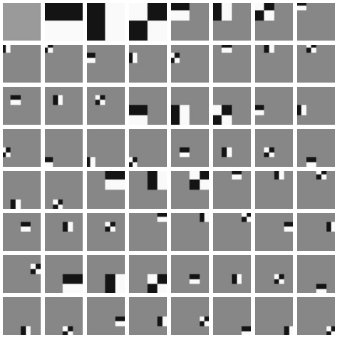
\includegraphics[width =
0.3\textwidth]{images/haar.jpg}}
\hspace{5mm}
\subfloat[gabor wavelet]{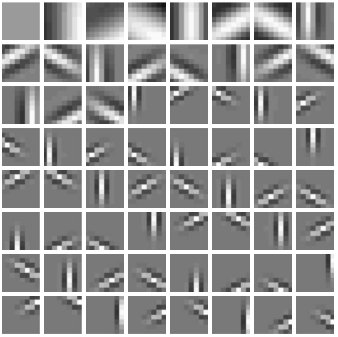
\includegraphics[width =
0.3\textwidth]{images/gabor.jpg}}
\caption[Generated dictionary atoms]{Generated dictionary atoms (Lewicki et
al.\cite{Lewicki1999})}
\label{fig:generated_atoms}
\end{figure}

\subsection{Learned atoms}
%\begin{quotation}
%A computer program is said to learn from experience E with respect to
%some class of tasks T and performance measure P, if its performance at tasks in
%T, as measured by P, improves with experience E.\footnote{Tom M. Mitchell}
%\end{quotation}
Recent research\cite{Chen1998,Aharon2006,Mairal2010} has shown that learned
dictionaries show better compression quality than small analytic
dictionaries. Rather than selecting an appropriate mathematical construct that
can reconstruct a certain group of signals close enough to the data, a subset of
the data or similar data is used as a training set to learn the dictionary
itself.
%Besides the construction of dictionaries from mathematical functions, machine
%learning can also be used to to generate dictionaries. 
Machine learning is such a process that is used to learn essential structures
from empirical data. In our case image samples are feed as training data into
machine learning algorithms.

\emph{Principal component analysis (PCA)} can be used as an approach to find
such dictionary atoms. As the principal components are orthogonal to each other,
PCA can only find a number of atoms that is lower or equal to the
dimension of the signal. When using these atoms for sparse coding we
are limited to a small range of possible atoms.

\paragraph{Redundancy} Unlike the PCA approach,
dictionary atoms learned with machine learning methods are not necessarily
orthogonal. In fact one benefit of the machine learning approach is to be able
to learn over-complete dictionaries with non-orthogonal basis atoms
(\prettyref{fig:learned_atoms}). This is where redundancy enters the game of
constructing dictionaries. Not in a way that multiple instance of the same atom
are part of the dictionary but in form of additional atoms resembling a
combination of other atoms from the dictionary. This can lead to less required
atoms and more sparseness in the coefficient vector $\vec{\alpha}$. Now a single
atom can achieve the same reconstruction as a former combination of several
atoms generated from orthogonal basis elements.

\begin{figure}
\centering
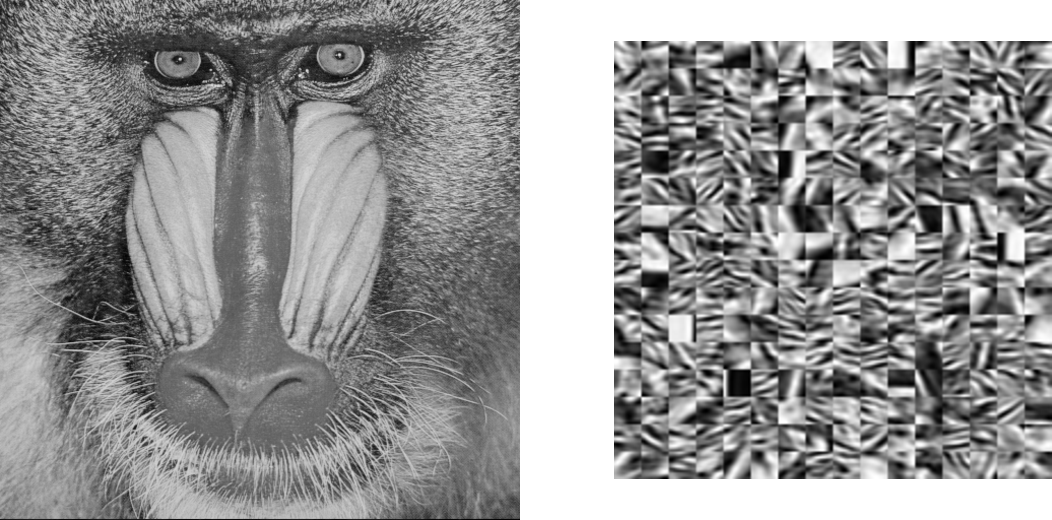
\includegraphics[width = 0.7\textwidth]{images/learned.pdf}
\caption[Learned redundant dictionary]{Source and learned redundant dictionary}
\label{fig:learned_atoms}
\end{figure}

Nevertheless redundancy can also be applied to designed dictionaries. For
example by adding rotated cosine atoms to a dictionary with a default
configuration of DCT basis elements.


\section{Learning}
%\cite{Olshausen1997,Lewicki2000,Aharon2006}
In the last decade several learning algorithms for over-complete dictionaries
have been proposed. 
%The typical formulation of learning a dictionary
%$\mat{D}$ is to minimize a loss function over a set of training samples
%$\mat{X}=[\vec{x}_1,...,\vec{x}_n]$.
The basic concept of following algorithms for learning
redundant dictionaries is to optimize a dictionary $\mat{D}$ in a
way that it minimizes a loss function over a set of training samples
$\mat{X}=[\vec{x}_1,...,\vec{x}_n]$.
%can sparsely reconstruct a set of training data $\mat{X}$ with
%minimal error.

\begin{equation*}
D \equiv \argmin_{\mat{D}} \sum_{i=1}^n \ell(\vec{x}_i,\mat{D})\label{eq:learn}
\end{equation*}
With a typical sparsity constraining loss function of:
\begin{equation*}
\ell(x,D) \equiv \min_{\vec{\alpha}} \lVert \vec{x} - \mat{D}\vec{\alpha}
\rVert^{2}_{2}  +  \lambda \lVert
\vec{\alpha}
\rVert_{0,1,2} 
\end{equation*}
%There are two major groups of algorithms for learning redundant dictionaries
%for sparse coding. 
There are two major groups of algorithms to achieve the desired optimization.
Learning dictionary elements from a fixed batch of training
signals and learning dictionary elements from a constant flow of data. The
latter enables to start the learning process before the actual training data is
known. An advantage that is used to learn from live data, for example video and
audio, or big data sets that would challenge the limits of a batch based
algorithm. We now introduce algorithms for both ways of learning.

\subsection{Batch algorithms}
Batch algorithms learn over-complete dictionaries from fixed batches of
training data. Besides the initial idea by Olshausen and Field in
1996\cite{Olshausen1996} Engan et al.\cite{Engan1999a} presented 
in 1999 the \emph{Method of optimal directions (MOD)} and recently the
\emph{Iterative least-square dictionary learning algorithm
(ILS-DLA)}\cite{Engan2007}. 


\subsubsection{K-SVD}
\label{sec:k-svd}
One of the most popular batch algorithms is the K-SVD presented by
Aharon et al. in 2006\cite{Aharon2006}. The \prettyref{alg:k-svd} learns a
dictionary
$\mat{D}$ from a set of training samples $\mat{X}$ by minimizing:
\begin{equation*}
\min_{\mat{D},\mat{A}} \lVert \mat{X} - \mat{D}\mat{A} \rVert^{2}_{F} \textrm{
s.t. }
\forall i : \lVert \vec{\alpha}_i \rVert_{0} \leq L
\end{equation*}
At the beginning the dictionary $\mat{D}$ gets initialized with either random
data or a random selection of elements from the training set. The main part of
the algorithm consists of two steps which are repeated for a fixed number of $T$
iterations or until convergence of $\mat{D}$. In the first step all samples of
training set $\mat{X}$ are sparse coded with the current dictionary $\mat{D}$
leading to sparse matrix $\mat{A}$. In the second step every dictionary atom
$\vec{d}_j$ of $\mat{D}$ is altered in a way that the reconstruction error of
$\mat{X}$ is minimized. 
\begin{equation*}
\min_{\vec{d}_j,\vec{a}_j} \lVert \vec{d}_j\vec{a}_j - \mat{E}_j \rVert^{2}_{F}
\textrm{ with }
\mat{E}_j = \sum_{l\neq j} \vec{d}_l\vec{a}_l^T - \mat{X}
\end{equation*} 
The trick of the update step is to consider only the signals in $\mat{X}$ which
use the atom $\vec{d}_j$. The problem gets then solved with a \emph{Singular
Value Decomposition (SVD)}. 
%The name K-SVD comes from $k$ times application of SVD in the update process
%(line \label{alg:k-svd_start} untill line \ref{alg:k-svd_end} in algorithm
%\ref{alg:k-svd}).

\begin{algorithm}[h]
\caption{K-SVD}
\label{alg:k-svd}
\begin{algorithmic}[1]
\REQUIRE $\mat{X} \in \mathbb{R}^{m \times k}, \mat{D}_0 \in \mathbb{R}^{m
\times p}, T \in \mathbb{N}, L \in \mathbb{N}$
\STATE $\mat{D	} \gets \mat{D}_0$
\FOR {$t = 1$ to $T$}
\STATE sparse code every $\vec{x}_t$ in $\mat{X}$ with $\mat{D}$:
\begin{equation}
\mat{A}[t] = \argmin_{\vec{\alpha}}\lVert
\vec{x}_t - \mat{D}\vec{\alpha}\rVert_2^2 \text{ s.t.}
\lVert\vec{\alpha}\rVert_0 \leq L
\end{equation}
\FOR {$j = 1$ to $p$}\label{alg:k-svd_start}
\STATE $\mat{D}[j] \gets 0$
\STATE $I \gets \{ i : \forall i : \mat{A}[i][j] \neq 0 \}$
\STATE $\mat{E} \gets \mat{X}_I - \mat{D}\mat{A}_I$
\STATE $\{\vec{d},\vec{g}\} \gets \argmin_{\vec{d},\vec{g}} \lVert \mat{E}-
\vec{d}\vec{g}^T \rVert_F^{2}$ s. t. $\lVert
\vec{d} \rVert_{2} = 1$
\STATE $\mat{D}[j] \gets \vec{d}$
\STATE $\mat{A}[j]_{I} \gets \vec{g}^T$
\ENDFOR\label{alg:k-svd_end}
\ENDFOR
\RETURN $\mat{D}$
\end{algorithmic}
\end{algorithm}

\subsection{Online algorithms}
In 2009 new training algorithms were presented enabling online learning of
dictionaries. In contrast to batch learning algorithms with a fixed training set
the new approaches enable learning with a constant flow of training data. This
is good for very large training sets or training data that is unknown at the
start of the training process.

One online algorithm is the \emph{Recursive least-square dictionary
learning algorithm (RLS-DLA)}. The algorithm was presented by Engan et al. in
2010\cite{Engan2010} and is a recursive modified version of the ILS-DLA
algorithm.

\subsubsection{Online dictionary learning}
\label{sec:mairal}
In 2009 Mairal et. al.\cite{Mairal2009} presented an online approach we call
\trainDL. The algorithm uses stochastic gradient descent to optimize
$\mat{D}$ (\prettyref{eq:learn}) with the loss function: 
\begin{equation*}
\ell(x,D) \equiv \min_{\vec{\alpha}} \frac{1}{2}\lVert \vec{x} -
\mat{D}\vec{\alpha} \rVert^{2}_{2}  +  \lambda \lVert
\vec{\alpha}
\rVert_{1} 
\end{equation*} 
%It is a minimization that uses
Like K-SVD the algorithm learns a dictionary $\mat{D}$ from a set of
training samples $\mat{X}$ and starts with a dictionary $\mat{D}$ with random
data or a random selection of elements from the training set. 

In each iteration $t$ \prettyref{alg:trainDL} draws a random sample
$\vec{x}_t$ from the training set $\mat{X}$ through a function
$p(\mat{X})$.
Then $\vec{x}_t$ gets sparse coded with $\mat{D}_{t-1}$ yielding
$\vec{\alpha}_t$. In each iteration \prettyref{alg:update} updates the
dictionary $\mat{D}$ with block-coordinate descent with $\mat{D}_{t-1}$ as warm
restart. 

The algorithm only requires to evaluate a single training sample in every
iteration $t$. Capturing previous coding informations in
$\mat{A}=\sum_{t=1}^T\vec{\alpha}_t\vec{\alpha}_t^T$, 
$\mat{B}=\sum_{t=1}^T\vec{x}_t\vec{\alpha}_t^T$ and $\mat{D}$.
This allows to scale up to large datasets of millions of training
samples or store $(\mat{A},\mat{B},\mat{D})$ and warm restart learning
with new samples.
% and being suitable for a large range of learning problems.
%Does it scale up to big dictionaries?

\begin{algorithm}[h]
\caption{ODL}
\label{alg:trainDL}
\begin{algorithmic}[1]
\REQUIRE $y \in \mathbb{R}^{m \times k},  p \left( \mat{X} \right),
\lambda \in
\mathbb{R}, \mat{D}_0 \in \mathbb{R}^{m \times p}, T \in \mathbb{N}$
\STATE $\mat{A}_0 \in \mathbb{R}^{p \times p} \gets  0, \mat{B}_0 \in
\mathbb{R}^{m \times p}\gets 0$
\FOR {$t = 1$ to $T$}
\STATE Draw $\vec{x}$ from $p(\mat{X})$.
\STATE Sparse code:
\begin{align*} 
\vec{\alpha}_t \equiv \argmin_{\vec{\alpha}\in\mathbb{R}^{p}}  \lVert \vec{x}_t
- \mat{D}_t\vec{\alpha} \rVert^{2}_{2}  +  \lambda \lVert \vec{\alpha}
\rVert_{1}
\end{align*}
\STATE $\mat{A}_t \gets \mat{A}_{t-1} +
\vec{\alpha}_t\vec{\alpha}_t^T$\label{alg:Aupdate}
\STATE $\mat{B}_t \gets \mat{B}_{t-1} +
\vec{x}_t\vec{\alpha}_t^T$\label{alg:Bupdate}
\STATE Compute $\mat{D}_t$ using \prettyref{alg:update}, with $\mat{D}_{t-1}$ as
warm restart 
\begin{equation}
\begin{split}
\mat{D}_t  & \equiv \argmin_{\mat{D} \in \mathbb{R}^{m x k}}  \frac{1}{t}
\sum_{i=1}^t
\left( \frac{1}{2} \lVert \vec{x}_i - \mat{D}\vec{\alpha}_i \rVert^{2}_{2}  + 
\lambda \lVert
\vec{\alpha}_i \rVert_{1} \right) \\
& = \argmin_{\mat{D} \in \mathbb{R}^{m x k}}  \frac{1}{t} \sum_{i=1}^t
\left( \frac{1}{2} Tr(\mat{D}^T\mat{D}\mat{A}_t) - Tr(\mat{D}^T\mat{B}_t)\right)
\label{eq:update}
\end{split}
\end{equation} 
\ENDFOR
\RETURN $\mat{D}_T$
\end{algorithmic}
\end{algorithm}
\begin{algorithm}[h]
\caption{Dictionary update}
\label{alg:update}
\begin{algorithmic}[1]
\REQUIRE $\mat{D}=[\vec{d}_1,...,\vec{d}_p] \in \mathbb{R}^{m \times p},
\mat{A}=[\vec{a}_1,...,\vec{a}_p] \in \mathbb{R}^{p \times p},
\mat{B}=[\vec{b}_1,...,\vec{b}_p] \in \mathbb{R}^{m \times p}$
\REPEAT
\FOR {$j = 1$ to $p$}
\STATE update the $j$-th column to optimize for \prettyref{eq:update}:
\begin{align*}
\vec{u}_j \gets
\frac{1}{\mat{A}[j,j]}\left(\vec{b}_j-\mat{D}\vec{a}_j\right)+\vec{d}_j \\
\vec{d}_j \gets \frac{1}{\max\left(\lVert \vec{u}_j \rVert_2,1\right)} \vec{u}_j
\end{align*}
\ENDFOR
\UNTIL convergence 
\RETURN $\mat{D}$
\end{algorithmic}
\end{algorithm}
In 2010 Mairal et al. \cite{Mairal2010} describe several modification to
their algorithm to improve speed and convergence. One speed optimization is to
sparse code mini-batches of $n$ samples instead of a single sample
in each iteration. This modification leads to line \ref{alg:Aupdate} and line
\ref{alg:Bupdate} of \prettyref{alg:trainDL} becoming:
\begin{align*}
\mat{A}_t \gets \mat{A}_{t-1} +
\frac{1}{n}\sum_{i=1}^{n}\vec{\alpha}_{t,i}\vec{\alpha}_{t,i}^T\\
\mat{B}_t \gets \mat{B}_{t-1} +
\frac{1}{n}\sum_{i=1}^{n}\vec{x}_{t,i}\vec{\alpha}_{t,i}^T
\end{align*}

\subsection{Learning for the task}
\label{sec:learnForTheTask}
``Please do not use the wrong dictionaries ...''
warns Guillermo Sapiro in his talk at the \emph{MIT CSAIL}.
It has been shown that learning specific for certain tasks can lead to the
best results. Based on this finding we will concentrate on a
specific class. We will focus on natural images from large image databases.
This means typically 1+ mega-pixel images with 3-channel RGB data found on image
hosting services such as flickr.com, twitpic.com, picasa.com among others.

\prettyref{sec:signal_representation} already describes that the learning
process is not limited to gray-scale oder RGB image signals. The presented
algorithms can be applied to different kinds of signals. Such as images in
other color spaces, low/high pass filtered sub-images or signals from another
domain like audio or text. 


\section{Related work}
\label{sec:related_dictionarie}


\paragraph{Training with a neural network} In his master thesis 
Krizhevsky\cite{Krizhevsky2009} is using a neural network to learn image
basis from a large set of tiny images. The resulting basis elements are similar
to wavelet filters.

\paragraph{Epitomes} In 2008 Wang et al.\cite{Wang2008a} presented
an approach that factors repeated content in images. The algorithm generates 
a map of affine transformations and an atlas texture with overlapping
regions of image content. This atlas is called epitome. The epitomes are also a
sort of dictionary and their affine transformations are
the corresponding sparse vectors. The technique is used for real-time synthesis
of textures with low memory consumption and fast reconstruction in hardware via
pixel shaders. They also presented some experiments for unified epitomes for
collections of images and possible application for larger sets of images. 

\paragraph{Multi-scale dictionaries}
Rather than encoding uniform blocks of an image this technique
codes different sized blocks (a multiple of the default block size). The
idea is that aligned smooth regions with low variance can be combined into big
blocks and coded with one rather than four sparse codes\cite{Mairal2007}.
%\Todo{optinal: picture with different scales}

\paragraph{Double sparsity}
In 2009 Rubinstein et al.\cite{Rubinstein2009} presented the idea of double
sparsity. Instead of dictionary consisting  of a collection of
learned atoms. This approach uses a second sparse coding step to encode
the atoms of a bigger dictionary $\vec{D}$ with the help of a smaller
dictionary $\vec{B}$ and a sparse matrix $\vec{A}$. Leading to a reconstruction
of $\mat{D}=\mat{B}\mat{A}$. 

\paragraph{Classification} When learning dictionaries
$(\mat{D}_{-},\mat{D}_{+})$ from individual groups of signal
$(\mat{S}_{-},\mat{S}_{+})$. A signal $\vec{x}$ can be classified
by $\min \left( \ell(\vec{x}\mat{D}_{-}),\ell(\vec{x}.\mat{D}_{+}) \right)$.
Examples for sparse coding being used for classification tasks can be found in
\cite{Grosse2007,Mairal2008,Mairal2008b,Bar2009}.

\paragraph{Hierarchy} Jenatton et al. showed in 2010\cite{Jenatton2010b} that
adding hierarchy to dictionaries can lead to faster coding of signals and
capture additional information about the learned dictionaries. While
dictionaries are learned the atoms are organized in a tree structure.
Under the constraint that child atoms require their parents being part of
the sparse selection. 








%\end{description}

